\section{Integration}

Recall: There are two different types of integral.  Suppose we have a function $f$.
  \begin{enumerate}
    \item The \emph{indefinite integral} of $f$ is a function $F$ such that
      \[
        \frac{dF}{dx} = f(x).
      \]
    We write
      \[
        F = \int f \, dx.
      \]
    This defines integration as the inverse of differentiation (antidifferentiation). $F$ is called the \emph{antiderivative} of $f$.
    \item The \emph{definite integral} is defined as the \emph{net signed area} between $f$ and the horizontal axis between $a$ and $b$. It is written
      \[
        \int_{a}^{b} f(x) \, dx.
      \]
  \end{enumerate}

You are probably used to using indefinite integrals to evaluate definite integrals, e.g.
  \begin{align*}
    \int_{0}^{\pi/2} \sin(x) dx &= [-\cos(x)]_{0}^{\pi/2} \\
    &= 0 - (-1) \\
    &= 1.
  \end{align*}
But why are we allowed to combine definite and indefinite integrals in this way?


\subsection{Fundamental Theorem of Calculus}

This theorem establishes the astonishing connection between indefinite and definite integrals.

\begin{theorem}

Let $f$ be a continuous function on $u \in [a,b]$.

\emph{Part A.}

The function $f$ has an antiderivative $g$ given by
\[
 g(x) = \int_{a}^{x} f(u) du
\]
(signed area between $a$ and $x$, definite integral).

\emph{Part B.}

Given any antiderivative $h$ of $f$,
\begin{eqnarray*}
 \int_{a}^{b} f(u) \, du &=& h(b) - h(a) \\
 &=& g(b) - g(a)\\
&=& \int f(x)dx \Big|_{x=b} - \int f(x)dx \Big|_{x=a}
 \end{eqnarray*}

 \end{theorem}

We don't have the formal mathematics required to prove this rigorously, and won't have until Semester 2 of Analysis 1.  Isaac Newton didn't have that formal mathematics yet either, so we (roughly) followed the method of justification he used in 1669.
% I could possibly add more detail about what he did - which I think was just a special case - after the "proof".


\begin{proof}[Justification of Part A]

We wish to differentiate
\[
 g(x) = \int_{a}^{x} f(u) \, du.
\]

Suppose $x$ changes by a small increment $\Delta x$.  The corresponding change in $g$ is $g(x + \Delta x) - g(x)$, so the average rate of change from $x$ to $x + \Delta x$ is
  \[
	  \frac{\Delta g}{\Delta x} = \frac{g(x + \Delta x) - g(x)}{\Delta x}.
	\]

As $\Delta x \rightarrow 0$, this approaches the derivative $\dfrac{dg}{dx}$.

Now, consider the diagram in figure (\ref{FTC_Proof}).

  \begin{figure}[H]
    \centering
    \def\svgwidth{0.8\columnwidth}
    \input{figures/latex/FTC_Proof.pdf_tex}
    \caption{The area \(g(x+\Delta x) = \text{area $A$} + \text{area $\Delta A$}\)}
    \label{FTC_Proof}
  \end{figure}

By definition of the definite integral defining $g$,
\[
g(x+\Delta x) = \text{area $A$} + \text{area $\Delta A$} = g(x) + \text{area $\Delta A$}.
\]

There is a point $\hat{x}$ with $x \leq \hat{x} \leq x + \Delta x$ such that $\Delta A = f(\hat{x})\Delta x$, as shown in figure (\ref{FTC_Proof}).  So
\begin{align*}
 g(x+\Delta x) - g(x) &= \text{area $\Delta A$} \\
 &= f(\hat{x})\Delta x
 \end{align*}

 Hence
 \[
  \dfrac{g(x+\Delta x) - g(x)}{\Delta x} = f(\hat{x})
 \]

 As $\Delta x \to 0$, $\hat{x} \to x$ (since it gets sandwiched between $x$ and $x + \Delta x$), so \(f(\hat{x}) \to f(x)\) and
 \[
  \dfrac{dg}{dx} = f(x)
 \]

Hence $g$ is an antiderivative for $f$.

(see Analysis 1 Semester 2 for a rigorous proof).

\end{proof}

Note that this result allows us to differentiate certain functions defined in terms of integrals.  Explicitly, the statement ``$g$ is an antiderivative for $f$'' means that
  \[
    \frac{dg}{dx} = \frac{d}{dx}\left(\int_{a}^{x} f(u) \, du\right) = f(x).
  \]
Notice also that the derivative of $g$ does not depend on the lower limit of the integral, $a$.  If we were to evaluate the integral and write an explicit expression for $g$ (assuming that this is possible), this constant $a$ would only contribute a constant term to that expression; the derivative of that constant term would therefore be $0$.



\begin{proof}[Justification of Part B]

Let $h$ be an antiderivative of $f$.

So
\begin{eqnarray*}
 && \dfrac{dh}{dx} = f = \dfrac{dg}{dx}\\
% && F(x) = \int_{0}^{x} f(u)du \\
 &\Longrightarrow& \dfrac{dh}{dx} - \dfrac{dg}{dx} = 0\\
 &\Longrightarrow& \dfrac{d}{dx}(h-g) = 0\\
 && \text{by linearity of derivative}\\
 &\Longrightarrow& h-g=c, \quad \text{constant}.
\end{eqnarray*}

Hence
\[
 h=g+c.
\]

Now
\begin{eqnarray*}
 \int_{a}^{b} f(x)dx &=& \int_{a}^{x} f(u)du \Big|_{x=b}\\
 &=& g(x)\Big|_{x=b} = g(b)
\end{eqnarray*}
\begin{eqnarray*}
 \int_{a}^{a} f(x)dx &=& g(a)=0,
\end{eqnarray*}
so
\begin{eqnarray*}
 \int_{a}^{b} f(x)dx &=&  g(b) - g(a)\\
 &=& (g(b)+c) - (g(a)+c)\\
 &=& h(b) - h(a)
\end{eqnarray*}

\end{proof}

% I'm not convinced that this corollary is useful or enlightening.
% I think the point is that it's common-ish for functions to be defined as integrals, and these functions are therefore easy to differentiate.
\begin{corollary}
 \[
  \dfrac{d}{dx} \int_{a(x)}^{b(x)} f(u)du = f(b) \dfrac{db}{dx} - f(a) \dfrac{da}{dx}
 \]
\end{corollary}

\begin{proof}
 Let $g(x)$ be an antiderivative of $f(x)$, so
 \[
  \dfrac{dg}{dx} = f(x)
 \]

 Then by Fundamental Theorem of Calculus,
 \[
  \int_{a(x)}^{b(x)} f(u)du = g(b(x))-g(a(x))
 \]

 \begin{eqnarray*}
  \Longrightarrow \quad \dfrac{d}{dx} \int_{a(x)}^{b(x)} f(u)du &=&
  \dfrac{dg}{db} \dfrac{db}{dx} - \dfrac{dg}{da} \dfrac{da}{dx}\\
  && \text{(chain rule)}\\ % This kind of typesetting is hideous.
  &=& f(b) \dfrac{db}{dx} - f(a) \dfrac{da}{dx}
 \end{eqnarray*}
\end{proof}



\subsection{Hyperbolic functions}

Hyperbolic functions are a type of function related to trigonometric functions.  We will use them to help us integrate various types of functions, using a technique called \emph{integration by substitution}, which we'll meet in the next section.

\begin{eqnarray*}
 && \cosh (x) = \dfrac{1}{2} (e^{x}+e^{-x})\\
 && \sinh (x) = \dfrac{1}{2} (e^{x}-e^{-x})\\
 && \tanh (x) = \dfrac{\sinh (x)}{\cosh (x)} = \dfrac{e^{x}-e^{-x}}{e^{x}+e^{-x}}
\end{eqnarray*}


\subsubsection*{Sketches}

What do $\cosh$ and $\sinh$ look like?

$\cosh(0)=1$

As $x \to \infty$, $\cosh(x) \to \infty$.

As $x \to -\infty$, $\cosh(x) \to \infty$.

$\cosh (x)>0$ $\forall x$.

\begin{figure}[H]
\centering
 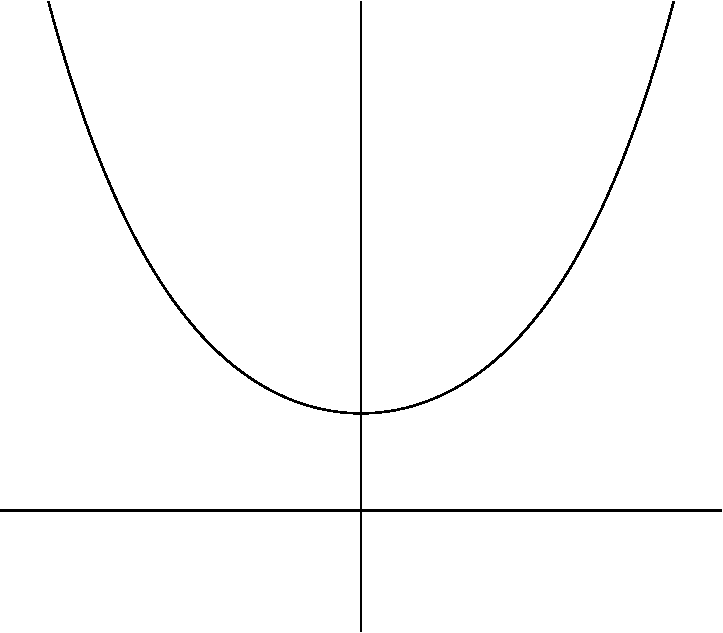
\includegraphics[width=0.6\textwidth]{cosh.pdf}
%\captionsetup{labelformat=empty}
\caption{$\cosh(x)$}
\end{figure}

Hanging chains (e.g. those in suspension bridges) have $\cosh$ shape, called a "catenary".

Soap bubbles between wands have a surface derived from the $\cosh$ shape.

$\sinh(0)=0$

As $x \to \infty$, $\sinh(x) \to \infty$.

As $x \to -\infty$, $\sinh(x) \to -\infty$.

\begin{figure}[H]
\centering
 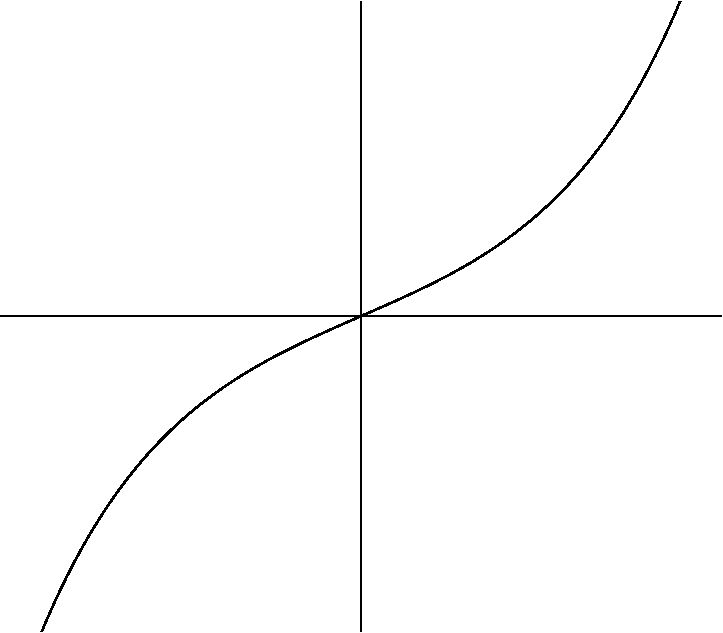
\includegraphics[width=0.6\textwidth]{sinh.pdf}
%\captionsetup{labelformat=empty}
\caption{$\sinh(x)$}
\end{figure}

$\tanh(0)=0$

As $x \to \infty$, $\tanh(x) \to 1$.

As $x \to -\infty$, $\tanh(x) \to -1$.

\begin{figure}[H]
\centering
 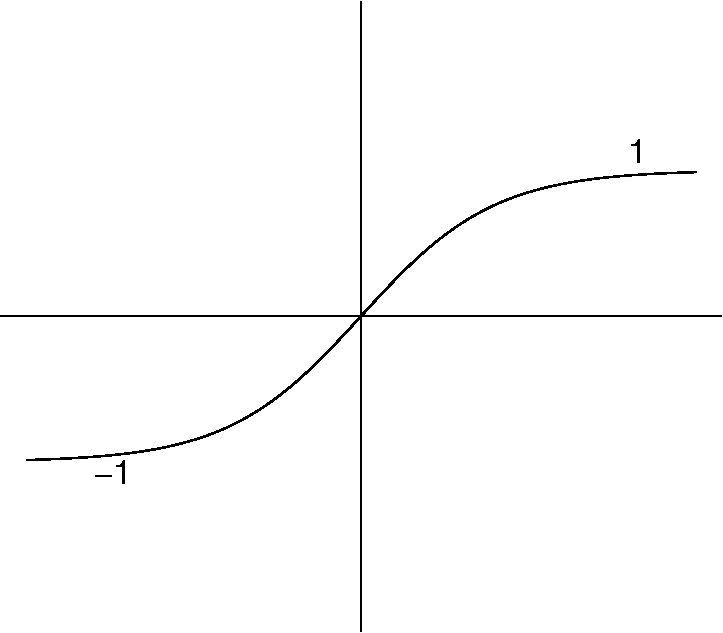
\includegraphics[width=0.6\textwidth]{tanh.pdf}
%\captionsetup{labelformat=empty}
\caption{$\tanh(x)$}
\end{figure}

\subsubsection*{Hyperbolic identities}

Hyperbolic functions satisfy identities similar to trigonometric identities.

\begin{examples}
  \quad
  \begin{enumerate}
		\item \(\cosh^{2}(x) - \sinh^{2}(x) = 1\) because
\begin{eqnarray*}
 \cosh^{2}(x) - \sinh^{2}(x)
 &=& \left(\dfrac{e^{x}+e^{-x}}{2}\right)^2
 - \left(\dfrac{e^{x}-e^{-x}}{2}\right)^2 \\
 &=& \dfrac{1}{4} \left(e^{2x} + 2 + e^{-2x}\right)
 - \dfrac{1}{4} \left(e^{2x} - 2 + e^{-2x}\right) \\
 &=& \dfrac{1}{2} + \dfrac{1}{2} = 1.
\end{eqnarray*}

Compare this with the trigonometric identity
\[
 \cos^{2}(x) + \sin^{2}(x) = 1.
\]
    \item \(1 - \tanh^2(x) = \sech^2(x).\)  Using \(\cosh^2(x) - \sinh^2(x) = 1\) and dividing through by \(\cosh^2(x)\) gives
		\[
		  \frac{\cosh^2(x)}{\cosh^2(x)} - \frac{\sinh^2(x)}{\cosh^2(x)} = \frac{1}{\cosh^2(x)},
		\]
		i.e. \(1 - \tanh^2(x) = \sech^2(x).\)
		
		Compare this with the trigonometric identity 
		  \[
			  1 + \tan^2(x) = \sec^2(x).
			\]
		\item The hyperbolic addition formula for \(\sinh\) is
		  \[
			  \sinh(x + y) = \sinh(x)\cosh(y) + \cosh(x)\cosh(y).
			\]
		The corresponding trigonometric identity is
		  \[
			  \sin(x + y) = \sin(x)\cos(y) + \cos(x)\cos(y).
			\]
		(See Exercise Sheet 1.)
		\item The hyperbolic addition formula for \(\cosh\) is
		  \[
			  \cosh(x + y) = \cosh(x)\cosh(y) + \sinh(x)\sinh(y).
			\]
		The corresponding trigonometric identity is
		  \[
			  \cos(x + y) = \cos(x)\cos(y) - \sin(x)\sin(y).
			\]
	\end{enumerate}
\end{examples}	

% I'm not sure that this Osborn's Rule stuff is strictly necessary, although the part about complex numbers is enlightening.

	In fact, \emph{Osborn's Rule} states that any trigonometric identity can be converted into a hyperbolic identity by
	  \begin{itemize}
			\item replacing trigonometric functions with their hyperbolic counterparts,
			\item swapping the sign of any product of two \(\sinh\)s.
		\end{itemize}
	Note: be careful with the second step, e.g.
	  \[
		  \tanh(x) = \frac{\sinh(x)}{\cosh(x)},
		\]
	so \(\tan^2(x)\) becomes \(-\tanh^2(x)\) (see Example 2).
	
	This arises because hyperbolic and trigonometric functions are related as follows:
	  \begin{align*}
		  \cosh(ix) & = \cos(x),  \\
			\cosh(x) & = \cos(ix),  \\
			\sinh(ix) & = i\sin(x),  \\
			\sinh(x) & = -i\sin(ix),
		\end{align*}
	where \(i^2 = -1\).
	
	This comes from Euler's relation:
	  \[
		  e^{i\theta} = \cos(\theta) + i\sin(\theta).
		\]
		
		
\subsubsection*{Geometric interpretation}

In trigonometric expressions such as \(\sin(\theta)\), \(\cos(\theta)\), etc., \(\theta\) can be interpreted as an angle.  Similarly, in \(\sinh(t)\) and \(\cosh(t)\), \(t\) can be interpreted as an area.

Since \(\cosh^2(t) - \sinh^2(t) = 1\), for any \(t\), the point \((x, y) = (\cosh(t), \sinh(t))\) lies on the curve \(x^2 - y^2 = 1\).  Then \(t\) corresponds to twice the area bounded by this curve, the \(x\)-axis, and the line from the origin to the point \((\cosh(t), \sinh(t))\), as shown in figure (\ref{inversehyperbolicarea}).

  \begin{figure}[H]
    \centering
    \def\svgwidth{0.3\columnwidth}
    \input{figures/latex/Inverse_Hyperbolic_Area.pdf_tex}
    \caption{\(t\) corresponds to twice the shaded area}
    \label{inversehyperbolicarea}
  \end{figure}

Because of this, the inverse hyperbolic functions are denoted \(\arsinh\), \(\arcosh\), etc. -- ``ar'' is an abbreviation of ``area''.


\subsubsection*{Differentiating hyperbolic functions}

Since hyperbolic functions are defined in terms of the exponential function, they are straightforward to differentiate.

\begin{align*}
  \frac{d}{dx}\sinh(x) & = \frac{d}{dx}\left(\frac{e^x - e^{-x}}{2}\right)  \\
                       & = \frac{e^x + e^{-x}}{2}  \\
                       & = \cosh(x)
\end{align*}

Similarly,
  \[
    \frac{d}{dx}\cosh(x) = \sinh(x),
  \]
  \[
    \frac{d}{dx}\tanh{x} = \frac{1}{\cosh^2(x)} = \sech^2(x).
  \]




\subsection{Integrating functions involving square roots}  \label{sect:sqrts}

Integrals involving functions with square roots often arise in mechanics.  In this section, we will investigate methods for integrating them using trigonometric and hyperbolic substitutions.

Recall that integration by substitution is a technique for evaluating integrals involving composite functions, using the formula
  \[
    \int f(g(x)) \dfrac{dg}{dx}dx = F(g(x)) + c,
  \]
derived from the chain rule for differentiation. (For a more detailed reminder of integration by substitution, see the additional notes on the course Moodle page.)


\begin{example}

Evaluate the integral
  \[
	  \int \sqrt{a^2 - x^2} \, dx,
	\]
where \(\left|x\right| < a\).

The integrand is a semicircle with radius \(a\).  To inform which choice of substitution to use, consider figure (\ref{semicircleintegralindefinite}).  The coordinates of any point \((x, \sqrt{a^2 - x^2})\) on the curve can be expressed in terms of \(\theta\), the angle between the \(y\)-axis and the line segment from the origin to that point, using trigonometric functions.

  \begin{figure}[H]
    \centering
    \def\svgwidth{0.55\columnwidth}
    \input{figures/latex/semicircleintegralindefinite.pdf_tex}
    \caption{Finding a substitution to integrate the curve \(\sqrt{a^2 - x^2}\)}
    \label{semicircleintegralindefinite}
  \end{figure}
	
From the right-angled triangle in figure (\ref{semicircleintegralindefinite}), we see that
  \[
    x  =  a \sin{\theta}.
  \]
We will use this for our substitution.  Then $\theta=\arcsin \left(\dfrac{x}{a}\right)$,\quad $\dfrac{dx}{d \theta} = a \cos(\theta)$, and
  \[
	  \sqrt{a^2 - x^2} = \sqrt{a^2 - a^2\sin^2(\theta)} = \sqrt{a^2\cos^2(\theta)} = a\cos(\theta),
	\]
using \(1 - \sin^2(\theta) = \cos^2(\theta)\); alternatively, one can deduce this from the right-angled triangle in figure (\ref{semicircleintegralindefinite}).

Thus the integral is
  \begin{align*}
    \int \sqrt{a^2 - x^2} \, dx & = \int a\cos(\theta) \times a\cos(\theta) \, d\theta \\
    & = \int a^2 \cos^2(\theta) \, d\theta \\
    & = \int \frac{a^2}{2}\left(1+\cos(2\theta)\right) \, d\theta \\
    & = \frac{a^2}{2} \theta + \frac{a^2}{4} \sin(2\theta) + c \\
    & = \frac{a^2}{2} \arcsin \left(\frac{x}{a}\right)+\frac{a^2}{4} \sin \left(2 \arcsin\left(\frac{x}{a}\right)\right) +c.\\
  \end{align*}

The second term can be simplified further: using the trigonometric identities
  \begin{align*}
	  \sin (2\theta) & = 2 \sin (\theta) \cos (\theta), \text{ and}   \\
		\cos (\theta) & = \sqrt{1-\sin^{2}(\theta)},
	\end{align*}
we have
  \begin{align*}
	  \sin \left(2 \arcsin\left(\frac{x}{a}\right)\right) & = 2 \sin \left(\arcsin\left(\frac{x}{a}\right)\right)\cos \left(\arcsin\left(\frac{x}{a}\right)\right)  \\
		& = 2\dfrac{x}{a} \left[1 - \sin^2 \left(\arcsin\left(\frac{x}{a}\right)\right) \right]^{1/2}  \\
		& = \dfrac{2x}{a} \sqrt{1-\dfrac{x^{2}}{a^{2}}}.
	\end{align*}
Thus
  \begin{align*}
    \int \sqrt{a^2 - x^2} \, dx & = \frac{a^2}{2} \arcsin \left(\frac{x}{a}\right)+\frac{a^2}{4} \sin \left(2 \arcsin\left(\frac{x}{a}\right)\right) +c.\\
		& = \frac{a^2}{2} \arcsin \left(\frac{x}{a}\right) + \frac{ax}{2} \sqrt{1-\dfrac{x^2}{a^2}} + c  \\
		& = \frac{a^2}{2} \arcsin \left(\frac{x}{a}\right) + \frac{x}{2} \sqrt{a^2 - x^2} + c.
  \end{align*}
	
For a geometric interpretation of this answer, consider the definite integral
  \begin{equation}  \label{semicircledefiniteexpression}
	  \int_0^b \sqrt{a^2 - x^2} \, dx = \frac{a^2}{2}\arcsin\left(\frac{b}{a}\right) + \frac{b}{2} \sqrt{a^2 - b^2},
	\end{equation}
where \(0 < b < a\).  This definite integral is the area shown in figure (\ref{semicircleintegraldefinite}), divided into two regions, \(R\) and \(S\).

  \begin{figure}[H]
    \centering
    \def\svgwidth{0.4\columnwidth}
    \input{figures/latex/semicircleintegraldefinite.pdf_tex}
    \caption{Definite integral of the curve \(\sqrt{a^2 - x^2}\)}
    \label{semicircleintegraldefinite}
  \end{figure}
	
The region \(R\) is a sector of a circle of radius \(a\) with angle \(\arcsin\left(\dfrac{b}{a}\right)\), and therefore has area
  \[
	  \frac{\pi a^2}{2\pi}\arcsin\left(\frac{b}{a}\right) = \frac{a^2}{2}\arcsin\left(\frac{b}{a}\right),
	\]
the first term in the expression for the definite integral (\ref{semicircledefiniteexpression}).

The region \(S\) is a triangle with base length \(b\) and height \(\sqrt{a^2 - b^2}\), and therefore has area
  \[
	  \frac{b}{2} \sqrt{a^2 - b^2},
	\]
the second term in the expression for the definite integral (\ref{semicircledefiniteexpression}).
\end{example}

There are a total of six similar cases (including this one) of integrals involving square roots:
  \begin{enumerate}
    \item $\sqrt{a^2 - x^2}$ \qquad ($\left|x\right| < a$)
    \item $\dfrac{1}{\sqrt{a^2 - x^2}}$ \qquad ($\left|x\right| < a$)
    \item $\dfrac{1}{\sqrt{a^2 + x^2}}$
    \item $\sqrt{a^2 + x^2}$
    \item $\dfrac{1}{\sqrt{x^2 - a^2}}$ \qquad ($\left|x\right| > a$)
    \item $\sqrt{x^2-a^2}$\qquad ($\left|x\right| > a$)
  \end{enumerate}

\begin{description}
\item[Case 2.]  This integrand includes the same square root expression as Case 1, so we use the same substitution,
  \[
    x  =  a \sin{\theta}.
  \]
With this substitution, $\theta=\arcsin \left(\dfrac{x}{a}\right)$ and $\dfrac{dx}{d \theta} = a \cos(\theta)$.

  \begin{align*}
    \int \dfrac{1}{\sqrt{a^2-x^2}} \, dx & = \int \dfrac{a \cos (\theta)}{\sqrt{a^2 - a^2\sin^2(\theta)}} \, d\theta  \\
		& = \int \dfrac{a \cos (\theta)}{a \cos(\theta)} \, d\theta  \\
		& = \int  d\theta \\
		& = \theta + c \\
		& = \arcsin\left(\dfrac{x}{a}\right) + c.
\end{align*}

\item[Case 3.] In Cases 1 and 2, we simplified the square root using the trigonometric identity
  \[
	  1 - \sin^2(\theta) = \cos^2(\theta).
	\]
In this case, we will use the hyperbolic identity
  \[
	  1 + \sinh^2(\theta) = \cosh^2(\theta)
	\]
in a similar way.  To do this, we use the substitution $x=a \sinh(\theta)$,  so
  \[
    \theta = \arcsinh \left(\dfrac{x}{a}\right), \qquad \dfrac{dx}{d\theta} = a \cosh(\theta).
  \]

\begin{eqnarray*}
 && \int \dfrac{dx}{\sqrt{a^2+x^2}} \\
 &=& \int \dfrac{a \cosh (\theta) d\theta}{\sqrt{a^2+a^2 \sinh^2(\theta)}} \\
 &=& \int \dfrac{a \cosh (\theta)}{a \cosh(\theta)}  d\theta \\
&=& \theta + c\\
&=& \arcsinh \left(\dfrac{x}{a}\right) + c\\
 \end{eqnarray*}

Recall from Exercise Sheet 1, question 4(a), that
\[
 \arcsinh (u) = \ln (u+\sqrt{u^2+1}),
\]
so
  \[
    \int \dfrac{dx}{\sqrt{a^2+x^2}} = \ln (x+\sqrt{x^2+a^2}) + c.
  \]

\item[Case 4, 5 and 6.] See Exercise Sheet 2.

\end{description}



\subsection{Integrating rational functions}

In this section, we will investigate methods for integrating rational functions.  A rational function is a function of the form
\[
 f(x) = \dfrac{a+bx+cx^{2} + \ldots + dx^{n}}{p + qx + rx^{2} + \ldots + sx^{m}}.
\]
They can be used to approximate many other functions.

\subsubsection*{Numerator $1$, denominator linear}

\begin{eqnarray*}
 f(x) &=& \dfrac{1}{ax+b}\\
 &=& \dfrac{1}{a} \times \dfrac{a}{ax+b}\\
 &=& \dfrac{1}{a} \dfrac{1}{g(x)} \dfrac{dg}{dx}\\
 \text{where } g(x) &=& ax+b
\end{eqnarray*}

So
\[
 \int f(x) dx = \dfrac{1}{a} \ln \left|ax+b\right| + c
\]

\subsubsection*{Numerator $1$, denominator quadratic}

\[
 f(x) = \dfrac{1}{ax^{2}+bx+c}
\]

We first consider two simpler cases, then show how the general case can be reduced to one of these.

\begin{examplesnumbered} \label{ex:quadraticdenominators}
 \quad
 \begin{enumerate}
  \item $f(x) = \dfrac{1}{a^{2} + x^{2}}$

         Substitution: let $x = a \tan(u)$, so that $u = \arctan \left(\dfrac{x}{a}\right)$.
				% This could do with more explanation about why I'm using that substitution.
				
				Then
				  \[
					  \frac{dx}{du} = a\sec^2(u),
					\]
				so
				  \begin{align*}
					  \int \frac{1}{a^2 + x^2} \, dx & = \int \frac{1}{a^2 + a^2\tan^2(u)} \times a\sec^2(u) \, du  \\
						& = \int \frac{a\sec^2(u)}{a^2(1 + \tan^2(u))} \, du  \\
						& = \int \frac{a\sec^2(u)}{a^2\sec^2(u)} \, du  \\
						& = \int \frac{1}{a} \, du  \\
						& = \frac{u}{a} + c  \\
						& = \frac{1}{a}\arctan\left(\frac{x}{a}\right) + c.
					\end{align*}

    \item $f(x) = \dfrac{1}{a^{2}-x^{2}} = -\dfrac{1}{x^{2}-a^{2}}$
		
		In this case, we have several options:
		  \begin{itemize}
				\item Use partial fractions:
				  \begin{align*}
					  f(x) & = \frac{1}{(a + x)(a - x)}  \\
						& = \frac{1}{2a}\left(\frac{1}{a + x} + \frac{1}{a - x}\right).
					\end{align*}
				\item If \(|x| < a\), use \(x = a\tanh(u)\).  Then \(a^2 - x^2 = a^2(1 - \tanh^2(u)) = a^2\sech^2(u)\).
				\item If \(|x| > a\), use \(x = a\coth(u)\), so \(a^2 - x^2 = a^2(1 - \coth^2(u)) = -a^2\cosech^2(u)\).
			\end{itemize}
		We will not cover the details of the substitutions here, since they are so similar to the \(\tan\) substitution in Case 1.
 \end{enumerate}

\end{examplesnumbered}


\subsubsection*{General quadratic denominator}

Given an integral with a general quadratic denominator,
    \begin{equation}  \label{eq:genquadraticdenom}
      \int \dfrac{dx}{ax^{2} + bx + c},
    \end{equation}
we perform the following steps:
  \begin{itemize}
		\item Complete the square in the denominator.
		\item Use a substitution to transform this into
		  \[
			  \int \frac{p}{u^2 \pm q^2} \, du,
			\]
		with \(p\) and \(q\) constant.
		\item If \(q = 0\), this can be integrated directly.
		\item Otherwise, integrate using the method from Case 1 or Case 2 from Examples~\ref{ex:quadraticdenominators}.
	\end{itemize}
	
	\begin{examplenumbered} \label{ex:genquaddenom}
	  Evaluate
		  \[
			  \int \frac{dx}{x^2 + 4x + 8} = \int \frac{dx}{(x + 2)^2 + 4}.
			\]
		We have completed the square in the denominator.  Now let \(u = x + 2\), so \(\dfrac{du}{dx} = 1\).  Then
		  \begin{align*}
			  \int \frac{dx}{(x + 2)^2 + 4} & = \int \frac{du}{u^2 + 2^2}  \\
				& = \frac{1}{2}\arctan\left(\frac{u}{2}\right) + c  \\
				& = \frac{1}{2}\arctan\left(\frac{x + 2}{2}\right) + c.
			\end{align*}
	\end{examplenumbered}
	
	For completeness, there follows an argument for evaluating \ref{eq:genquadraticdenom} for general values of \(a\), \(b\) and \(c\). 	Since this is notationally fiddly, but not substantially more complicated than the previous example, this general argument will not be covered in the lectures.

The denominator is
\begin{eqnarray}
 ax^{2} + bx + c &=& a \left[x^{2}+ \left(\dfrac{b}{a}\right)x + \left(\dfrac{c}{a}\right)\right]\notag\\
 &=& a \left[\left(x+ \dfrac{b}{2a}\right)^{2} + \dfrac{c}{a}-\dfrac{b^{2}}{4a^{2}}\right]\notag\\
  &=& a \left[\left(x+ \dfrac{b}{2a}\right)^{2} + \dfrac{4ac-b^{2}}{4a^{2}}\right]\label{eq4.5}.
\end{eqnarray}

To simplify the notation, write $\Delta=4ac-b^{2}$, which is a constant.  We make the substitution $u=x+\dfrac{b}{2a}$, so $\dfrac{du}{dx}=1$.

Then, from \eqref{eq4.5},
\[
 ax^{2} + bx + c = a \left[u^{2}+ \dfrac{\Delta}{4a^{2}}\right]
\]
so
\[
 \int \dfrac{dx}{ax^{2}+bx+c} = \dfrac{1}{a} \int \dfrac{du}{u^{2} + \dfrac{\Delta}{4a^{2}}}
\]

If $\Delta>0$, use $\tan$ substitution for $\dfrac{1}{q^2 + u^{2}}$ with $q = \dfrac{\sqrt{\Delta}}{2a}$.

If $\Delta<0$, use partial fractions or a $\tanh$ or \(\coth\) substitution for $-\dfrac{1}{q^2 - u^{2}}$ with $q = \dfrac{\sqrt{-\Delta}}{2a}$.

If $\Delta=0$, the integral does not require a substitution.

\subsubsection*{General quadratic numerator and denominator}

Given an integral with a general quadratic numerator and denominator,
\[
 \int \dfrac{px^{2} + qx + r}{ax^{2} + bx + c} dx,
\]
we use a series of transformations to break this into expressions that we already know how to integrate.

  \begin{example}
	  Evaluate
		  \[
			  \int \frac{2x^2 + 6x + 15}{x^2 + 4x + 8} \, dx.
			\]
		We write \(f(x)\) for the integrand.  First, we manipulate the integrand to remove the \(x^2\) term from the numerator:
		  \begin{align*}
			  f(x) & = \frac{2x^2 + 6x + 15}{x^2 + 4x + 8}  \\
				& = \frac{2(x^2 + 4x + 8) - 2x - 1}{x^2 + 4x + 8}  \\
				& = 2 - \frac{2x + 1}{x^2 + 4x + 8}.
			\end{align*}
		We cannot do the same to simplify the linear over quadratic term; however, this would be straightforward to integrate if the numerator was the derivative of the denominator.
		
		Observe: \(\dfrac{d}{dx}(x^2 + 4x + 8) = 2x + 4\), so we write
		  \begin{align*}
			  f(x) & = 2 - \frac{2x + 4 - 3}{x^2 + 4x + 8}  \\
				& = 2 - \frac{2x + 4}{x^2 + 4x + 8} + \frac{3}{(x + 2) + 4}.
			\end{align*}
			
	We have broken \(f(x)\) into three terms that we can integrate.  Notice that the third term is a multiple of the function from Example~\ref{ex:genquaddenom}.  We get
	\[
	  \int f(x) \, dx = 2x - \ln(x^2 + 4x + 8) + \frac{3}{2}\arctan\left(\frac{x + 2}{2}\right) + c.
	\]			
  \end{example}
	
	As before, the fully general case will not be covered in lectures, but is included here for completeness:
\begin{eqnarray*}
&& \int \dfrac{px^{2} + qx + r}{ax^{2} + bx + c} dx \\
 &=& \int \dfrac{\dfrac{p}{a} (ax^{2} + bx + c)}{ax^{2} + bx + c}
 + \dfrac{qx + r - \left[\dfrac{pb}{a}x - \dfrac{pc}{a}\right]}{ax^{2} + bx + c} dx\\
&=& \dfrac{px}{a} + \int \dfrac{ex+f}{ax^{2}+bx+c} dx \\
&=& \dfrac{px}{a} + \int \dfrac{\dfrac{e}{2a} (2ax+b)}{ax^{2}+bx+c} + \dfrac{f-\left[\dfrac{be}{2a}\right]}{ax^{2}+bx+c} dx\\
&=& \dfrac{px}{a} + \dfrac{e}{2a} \ln \left|ax^{2}+bx+c\right| + \left(f-\dfrac{be}{2a}\right) \int \dfrac{dx}{ax^{2}+bx+1}.
\end{eqnarray*}



\subsection{Reciprocals of trigonometric functions}

The methods in the previous have uses beyond integrating rational functions.  Certain other integrals can be evaluated by making a careful choice of substitution that converts the integrand into a rational function.

In the following examples we look at substitution that does this for integrals involving trigonometric functions.  The substitution we will use is not at all obvious substitution -- it was described by Michael Spivak (author of one of the recommended books for Analysis 1) as ``the world's sneakiest substitution''.

\begin{example}
Evaluate $\displaystyle\int \dfrac{d \theta}{2+\sin(\theta)+\cos(\theta)}$.

We will use the substitution $t=\tan \left(\dfrac{\theta}{2}\right)$.  Consider the right-angled triangle


\begin{center}
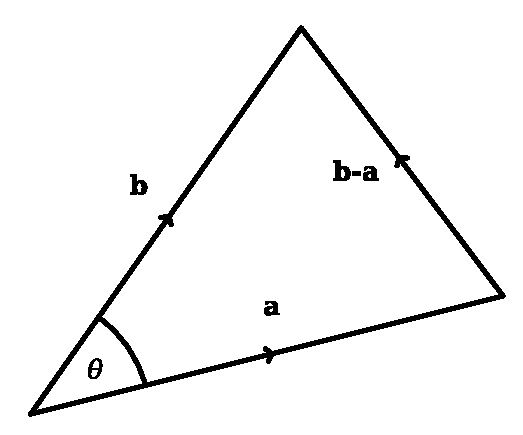
\includegraphics[width=0.45\textwidth]{triangle.pdf}
\end{center}

We have
\begin{eqnarray*}
 \sin \left(\frac{\theta}{2}\right) & = & \dfrac{t}{\sqrt{1+t^2}}, \\
 \cos \left(\frac{\theta}{2}\right) & = & \dfrac{1}{\sqrt{1+t^2}},
\end{eqnarray*}
so
\begin{eqnarray*}
 \sin(\theta) & = & 2 \sin \left(\frac{\theta}{2} \right) \cos
\left(\frac{\theta}{2} \right) \\
&= & \frac{2t}{(1+t^2)} \\
 \cos (\theta)& = & \cos^2 \left(\frac{\theta}{2} \right) -
\sin^2 \left(\frac{\theta}{2} \right) \\
& = &
\frac{(1-t^2)}{(1+t^2)}
\\
 \tan(\theta) & = & \frac{2 t}{(1-t^2)}
\end{eqnarray*}

Also
\begin{eqnarray*}
\frac{dt}{d \theta} & =& \frac{1}{2} \sec^2
\left(\frac{\theta}{2} \right) \\
& = & \frac{t^2+1}{2},
\end{eqnarray*}
so
\[
  \frac{d \theta}{dt}  =  \frac{2}{1+t^2}
\]

Observe that this substitution will convert any integral involving only $\sin$, $\cos$ and $\tan$, combined by addition, multiplication and division, into the integral of a rational function.  We now use it to evaluate the integral in our example.

Then
\begin{align*}
& \phantom{=} \int \frac{d \theta}{2+\sin(\theta)+\cos(\theta)}  \\
& = \int \frac{1}{2 + \left( \frac{2t}{1 + t^2} \right) + \left( \frac{1 - t^2}{1 + t^2} \right)} \times \frac{2}{1 + t^2} dt \\
& = \int\frac{2 dt}{t^2+2t+3} \\
& = \int \frac{2 dt}{(t+1)^2 + 2} \\
& = \sqrt{2} \arctan \left(\frac{1+t}{\sqrt{2}}\right) + c \\
& = \sqrt{2} \arctan \left(\frac{1+\tan(\theta/2)}{\sqrt{2}}\right) + c.
\end{align*}

\end{example}

% I have never done this example in the lectures and have omitted it for now.
% It would be nice on an exercise sheet, but there probably isn't space.

%\begin{example}
 %Suppose the radius $r$ of the orbit of a planet around its sun satisfies
 %\[
 %r=\dfrac{\ell}{1+k \cos(\theta)}, \qquad 0 \leq k \leq 1, \qquad l > 0.
 %\]
%
 %\begin{center}
  %\includegraphics[width=0.7\textwidth]{trig4.pdf}
 %\end{center}
%
 %What is the mean distance from the sun?  To find it we integrate the distance over all angles $\theta$, then divide by sum of all angles, $2\pi$.  We will be using the subtitution $t=\tan(\theta/2)$, so we must integrate from $\pi$ to $\pi$, since this substitution gives $\theta = 2\arctan(t)$, and
  %\[
    %- \frac{\pi}{2} < \arctan(t) < \frac{\pi}{2}
  %\]
%for all real numbers $t$.
%
 %\[
  %\overline{r} = \dfrac{1}{2\pi} \int_{-\pi}^{\pi} \dfrac{\ell}{1+k \cos(\theta)} d\theta
 %\]
%
%Let $t=\tan\left(\dfrac{\theta}{2}\right)$.  Then
  %\begin{align*}
    %\overline{r} & = \frac{1}{2\pi} \int_{\pi}^{\pi} \frac{l}{1 + k\cos(\theta)} \, d\theta  \\
    %& = \frac{l}{2\pi} \int_{-\infty}^{\infty} \frac{l}{1 + k\left( \frac{1 - t^2}{1 + t^2} \right)} \times \frac{2}{1 + t^2} \, dt  \\
    %& = \frac{l}{\pi} \int_{-\infty}^{\infty} \frac{1}{1 + t^2 + k - kt^2} \, dt  \\
    %& = \frac{l}{\pi} \int_{-\infty}^{\infty} \frac{1}{(1 - k)t^2 + (1 + k)} \, dt.
  %\end{align*}
%Now let $u = \sqrt{1 - k}t$, write $a = \sqrt{1 + k}$.  Then
  %\begin{align*}
    %\overline{r} & = \frac{l}{\pi} \int_{\pi}^{\pi} \frac{1}{u^2 + a^2} \times \frac{1}{\sqrt{1 - k}} \, du  \\
    %& = \frac{l}{\pi\sqrt{1 - k}} \left[ \frac{1}{a} \arctan\left( \frac{u}{a} \right) \right]_{-\infty}^{\infty}  \\
    %& = \frac{l}{\pi\sqrt{1 - k}\sqrt{1 + k}} \left[\frac{\pi}{2} - \left( - \frac{\pi}{2} \right)\right]  \\
    %& = \frac{l}{\sqrt{1 - k^2}}.
  %\end{align*}
%
%\end{example}




\subsection{Reduction formulae}

Recall that integration by parts is a technique for evaluating integrals involving products of functions using the formula
  \[
    \int u \frac{dv}{dx} \, dx   =   u v - \int v \frac{du}{dx} \, dx,
  \]
which is derived from the product rule for differentiation.  (For a more detailed reminder of integration by parts, see the additional notes on the course Moodle page.)

Sometimes complicated integrals can be reduced to simpler expressions by successive application of integration by parts, giving a type of formula called a \emph{reduction formula}.
% Not convinced by the wording of this last sentence.

\begin{examples}
\quad

\begin{enumerate}

\item $\displaystyle\int \left(\ln(x)\right)^n \, dx$,\quad $n=0,1,2,\dotsc$

Write
  \begin{align*}
    I_n & = \int \left(\ln(x)\right)^n \, dx  \\
    & = \int 1 \times (\ln(x))^ndx \\
	\end{align*}
Let
  \[
	  u = (\ln(x))^n, \quad \frac{dv}{dx} = 1,
	\]
so
  \[
	  \frac{du}{dx} = \frac{n(\ln(x))^{n - 1}}{x}, \quad v = x.
	\]
Then, using integration by parts,
	\begin{align*}
    I_n & = x (\ln(x))^n - \int x \frac{n (\ln(x))^{n-1}}{x} dx \\
    & = x (\ln(x))^n - n \int (\ln(x))^{n-1} dx \\
    I_n & = x (\ln(x))^n - n I_{n-1}
  \end{align*}
	
This formula allows us to evaluate \(I_n\) for a given value of \(n\) -- provided we also do so for all lower values of \(n\):
  \begin{align*}
    I_3 & = x[\ln(x)]^3 - 3 I_2, \\
    I_2 & = x [\ln(x)]^2 - 2 I_1, \\
    I_1 & = x \ln(x) - I_0, \\
    I_0 & = \int 1dx  =  x,
	\end{align*}
so
	\begin{align*}
    I_1 & = x\ln(x) - x, \\
    I_2 & = x[\ln(x)]^2 - 2 x \ln(x) + 2x, \\
    I_3 & = x[\ln(x)]^3 - 3 x [\ln(x)]^2 + 6 x \ln(x) - 6 x\ln(x) - 6x + C.
  \end{align*}

\item $I_n = \displaystyle\int \sin^n(x)dx$,\quad $n=0,1,2, \dotsc$
  
	Write this as
  \[
    I_n = \int \sin(x) \sin^{n-1}(x) \, dx
  \]
Let 
  \[
	  u = \sin^{n-1}(x), \quad \frac{dv}{dx} = \sin(x),
	\]
so
  \[
	  \frac{du}{dx} = (n - 1)\cos(x)\sin^{n-2}(x), \quad v = -\cos(x).
	\]
Then, using integration by parts,
  \begin{align*}
    I_n & =  -\cos(x)\sin^{n-1}(x) + \int \cos(x) (n-1)\cos(x) \sin^{n-2}(x)dx  \\
    & = -\cos(x)\sin^{n-1}(x) + (n-1) \int \cos^2(x)\sin^{n-2}(x)dx
  \end{align*}
But $\cos^2(x) = 1 - \sin^2 (x)$
  \begin{align*}
    I_n & = -\cos(x)\sin^{n-1}(x) + (n-1)\int \sin^{n-2}(x)dx - (n-1)\int \sin^n (x)dx  \\
    & = -\cos(x)\sin^{n-1}(x) + (n-1) I_{n-2} - (n-1)I_n.
	\end{align*}
	
	Rearranging this gives
	  \[
		  I_n = \frac{1}{n} \left[-\cos(x)\sin^{n-1}(x)\right] + \frac{n-1}{n} I_{n-2}.
		\]
  
	We can use this calculate any \(I_n\).  For example, when \(n = 3\), we get
	\begin{align*}
    I_3 & = \frac{1}{3} \left[-\cos(x)\sin^2(x)\right] + \frac{2}{3}I_1, \\
    I_1 & = \int \sin(x)dx  =  -\cos(x) + c, \\
    \therefore \quad I_3 & = -\frac{1}{3} \cos(x)\sin^2(x) - \frac{2}{3}\cos(x) + c.
  \end{align*}


% Removed this example -- it will be Exercise Sheet material only from now on.

%\item $\displaystyle\int \dfrac{dx}{(1+x^2)^{n}}$.
%
%\begin{eqnarray*}
%I_n &  = & \int \frac{dx}{(1+x^2)^n} \\
%I_1 &  = & \int \frac{dx}{1+x^2}  =  \int \frac{1 \times dx}{1+x^2} \\
%&  = & \frac{x}{1 + x^2} + \int \frac{2 x^2}{(1+x^2)^2}dx \\
%I_1 &  = & \frac{x}{1 + x^2} + 2 \int \frac{x^2 + 1 - 1}{(1 +
%x^2)^2} dx \\
%I_1 &  =  &\frac{x}{1 + x^2} + 2 \int \frac{dx}{(1 +
%x^2)}  - 2 \int \frac{dx}{(1 + x^2)^2} \\
%I_1 &  = & \frac{x}{1+x^2} + 2 I_1 - 2I_2 \\
%\therefore \qquad I_2 &  = & \frac{1}{2}
%\left[\dfrac{x}{1+x^2}\right] + \dfrac{I_1}{2} \\
%I_1 &  = & \arctan(x) + c
%\end{eqnarray*}
%
%Now find $I_{n+1}$ given $I_{n}$ (See Exercie Sheet 3).
% Check which worksheet it is once the worksheets are ready!

\end{enumerate}
\end{examples}


\subsection{Arc length and surface areas of revolution}


\subsubsection*{Arc length} 
We often need to know the length of a curve between two points,
e.g.\ what is the length of the ropes holding Clifton suspension bridge
(see Exercise Sheet 3).

\textbf{Idea. } Given a curve $y=y(x)$

  \begin{figure}[H]
    \centering
   % \def\svgwidth{0.4\columnwidth}
    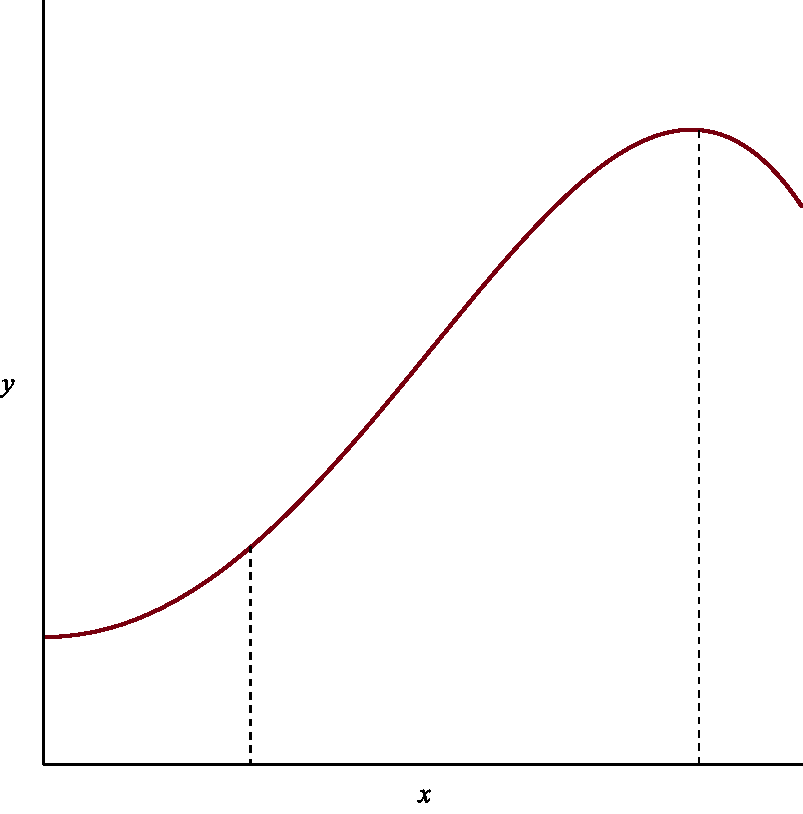
\includegraphics[width=0.6\textwidth]{arclength1.pdf}
  \end{figure}


Let $S$ be the arc length
and  $\Delta S$ a short section of it.

  \begin{figure}[H]
    \centering
   % \def\svgwidth{0.4\columnwidth}
    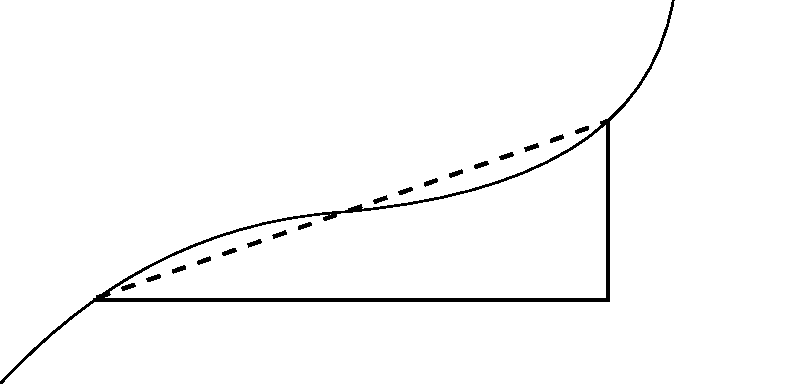
\includegraphics[width=0.6\textwidth]{arclengthdx.pdf}
  \end{figure}


By Pythagoras' Theorem,
\begin{eqnarray*}
\Delta S^2&\approx& \Delta x^2+\Delta y^2\\
\Rightarrow
\left(\dfrac{\Delta S}{\Delta x}\right)^2&\approx&1+\left(\dfrac{\Delta y}{\Delta x}\right)^2
\end{eqnarray*}
As $\Delta x\to0$ this becomes an identity
\begin{eqnarray*}
\left(\dfrac{d S}{d x}\right)^2&=&1+\left(\dfrac{d y}{d x}\right)^2\\
\Rightarrow
\dfrac{d S}{d x}&=&\sqrt{1+\left(\dfrac{d y}{d x}\right)^2}
\end{eqnarray*}
The arclength between $x=a$ and $x=b$ is then
\begin{eqnarray*}
S(a,b)&=&\int_a^b\dfrac{d S}{d x}dx\\
&=&\int_a^b\sqrt{1+\left(\dfrac{d y}{d x}\right)^2}dx.
\end{eqnarray*}

\begin{example}

Find the arc length of the graph of the function
\[
y=f(x)=\dfrac{x^3}6+\dfrac1{2x}
\]
on the interval $\left(\dfrac12,2\right)$.

Sketch the graph of $f(x)$ for $x>0$:

If $x=0$, $y$ is undefined.

We have $y=0$ if $\dfrac{x^3}6=-\dfrac1{2x}\Rightarrow x^4=-3$, hence never.

As $x\to0_+$, $y\to\infty$.
\\
As $x\to\infty$, $y\to\infty$ as well.

\begin{figure}[H]
\centering
 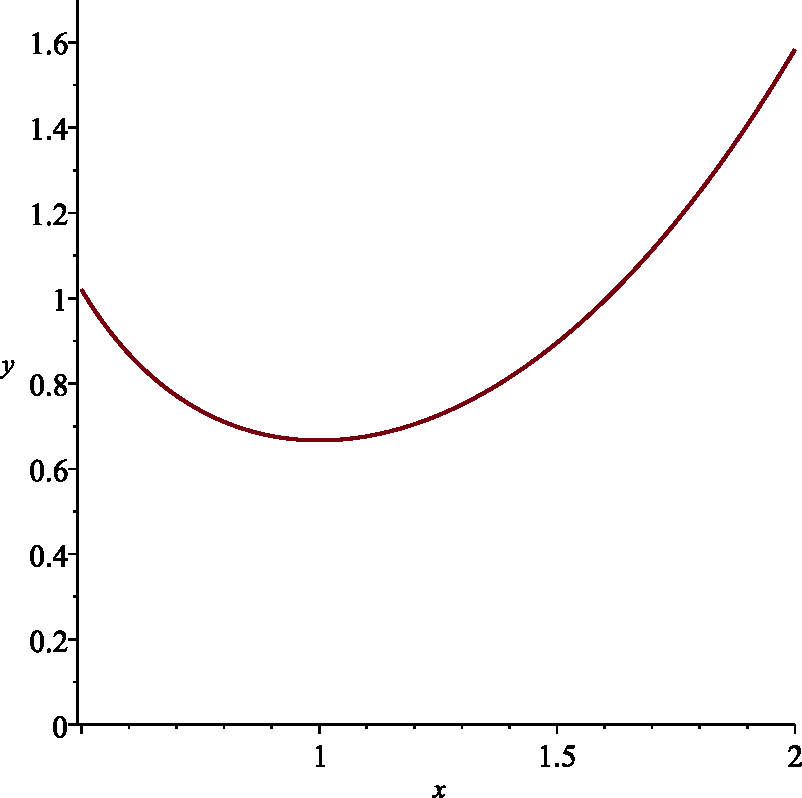
\includegraphics[width=0.5\textwidth]{arclengthexample.pdf}
%\captionsetup{labelformat=empty}
\end{figure}

Also, 
\[
\dfrac{d y}{d x}=\dfrac{3x^2}6-\dfrac1{2x^2}=\dfrac12\left(x^2-\dfrac1{x^2}\right).
\]
So
$\dfrac{d y}{d x}=0$ when $x^2-\dfrac1{x^2}=0
\Rightarrow
x^4=1
\Rightarrow
x=\pm1$.

Now, the arc length is
\[
S\left(\dfrac12,2\right)=\int_{\frac12}^2\sqrt{1+\left(\dfrac{d y}{d x}\right)^2}dx,
\]
with
\begin{eqnarray*}
1+\left(\dfrac{d y}{d x}\right)^2
&=&1+\dfrac14\left(x^2-\dfrac1{x^2}\right)^2\\
&=&1+\dfrac14\left(x^4-2+\dfrac1{x^4}\right)\\
&=&\dfrac14\left(x^4+2+\dfrac1{x^4}\right)\\
&=&\dfrac14\left(x^2+\dfrac1{x^2}\right)^2.
\end{eqnarray*}
Thus,
\begin{eqnarray*}
S\left(\dfrac12,2\right)
&=&\int_{\frac12}^2\dfrac12\left(x^2+\dfrac1{x^2}\right)dx\\
&=&\dfrac12\left[\dfrac{x^3}3-\dfrac1{x}\right]_{\frac12}^2=\dfrac{33}{16}.
\end{eqnarray*}
\end{example}

\begin{example}

It can be shown that a hanging chain forms a curve (see Exercise Sheet 4 Q.5)
\[
y=\cosh(x).
\]
The arc length on the interval $\left(-a,a\right)$ is
\begin{eqnarray*}
S\left(-a,a\right)&=&\int_{-a}^a\sqrt{1+\left(\dfrac{d y}{d x}\right)^2}dx\\
&=&\int_{-a}^a\sqrt{1+\sinh^2(x)}dx\\
&=&\int_{-a}^a\cosh(x)dx
=%\\&=&
\Big[\sinh(x)\Big]_{-a}^a=2\sinh(a).
\end{eqnarray*}
\end{example}

\textbf{Warning. } Calculating arc length often leads to integrals we cannot evaluate, e.g. $y(x)=\sin(x)$ yields
\[
S=\int_a^b\sqrt{1+\cos^2(x)} \, dx=???
\]

\subsubsection*{Surface areas of revolutions} 

Given a curve $y(x)$ we can generate a surface (of revolution) by rotating the curve about the $x$-axis.

What is the area of such a surface?

\textbf{Idea. } 
Split the shell into thin strips

  \begin{figure}[H]
    \centering
   % \def\svgwidth{0.4\columnwidth}
    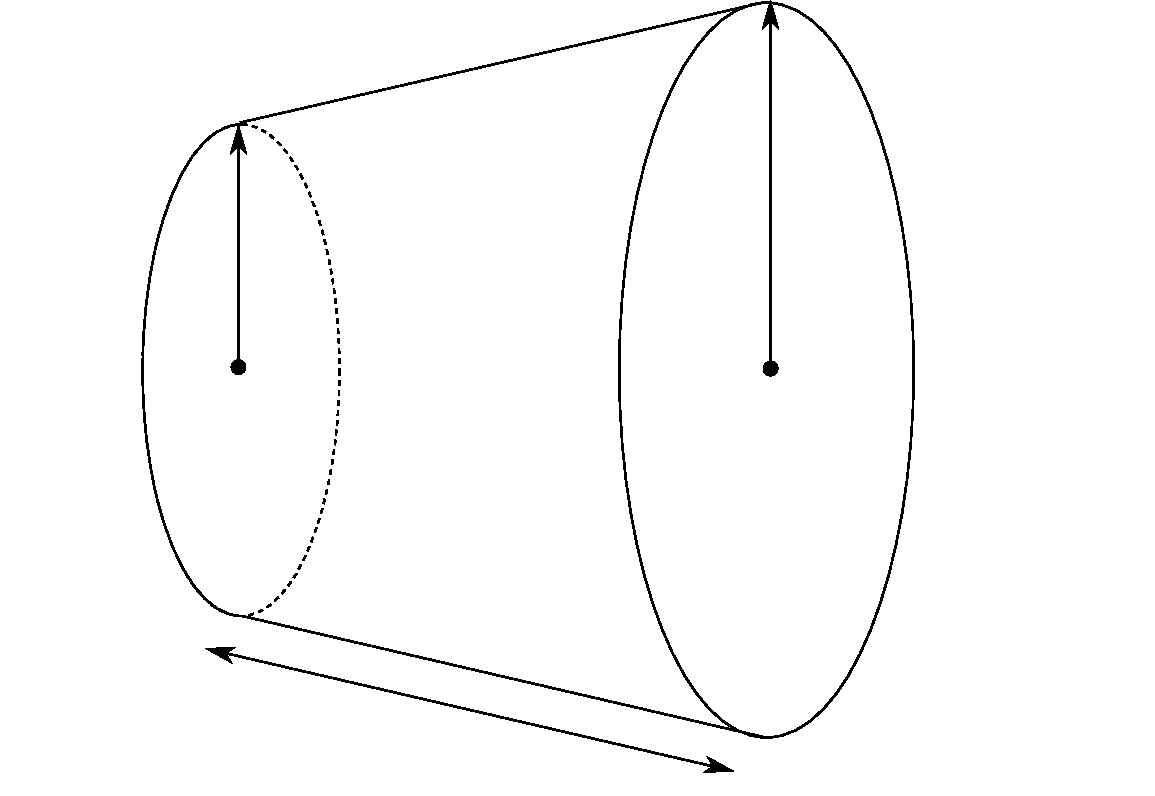
\includegraphics[width=0.6\textwidth]{frustum.pdf}
  \end{figure}

The area of the shell of a {\bf Conical Frustum} is $A=\pi (r_1+r_2)L$.

Thus, the area of the strip is approximately 
(set $r_1=y, r_2=y+\Delta y, L=\Delta S$)

\begin{eqnarray*}
\Delta A&\approx&\pi (y+(y+\Delta y))\cdot\Delta S\\
\Rightarrow\ \dfrac{\Delta A}{\Delta x}&=&2\pi \left(y+\frac12\Delta x\dfrac{\Delta y}{\Delta x}\right)\cdot\dfrac{\Delta S}{\Delta x}.
\end{eqnarray*}
As $\Delta x\to0$ 
$$
\dfrac{dA}{dx}=2\pi y\dfrac{dS}{dx}
\text{\qquad  as\quad} \dfrac{\Delta y}{\Delta x}\to\dfrac{dy}{dx} \text{ stays bounded.}
$$
Hence, using the previous arclength formula
\begin{eqnarray*}
A(a,b)&=&\int_a^b\dfrac{dA}{dx}dx
=%\\&=&
2\pi \int_a^b y\sqrt{1+\left(\dfrac{d y}{d x}\right)^2}\ dx.
\end{eqnarray*}


\begin{example}

Consider the curve $y=\sqrt{1+x^2}$, creating a hyperboloid of revolution (the flipped cooling tower).

  \begin{figure}[H]
    \centering
    \def\svgwidth{0.5\columnwidth}
    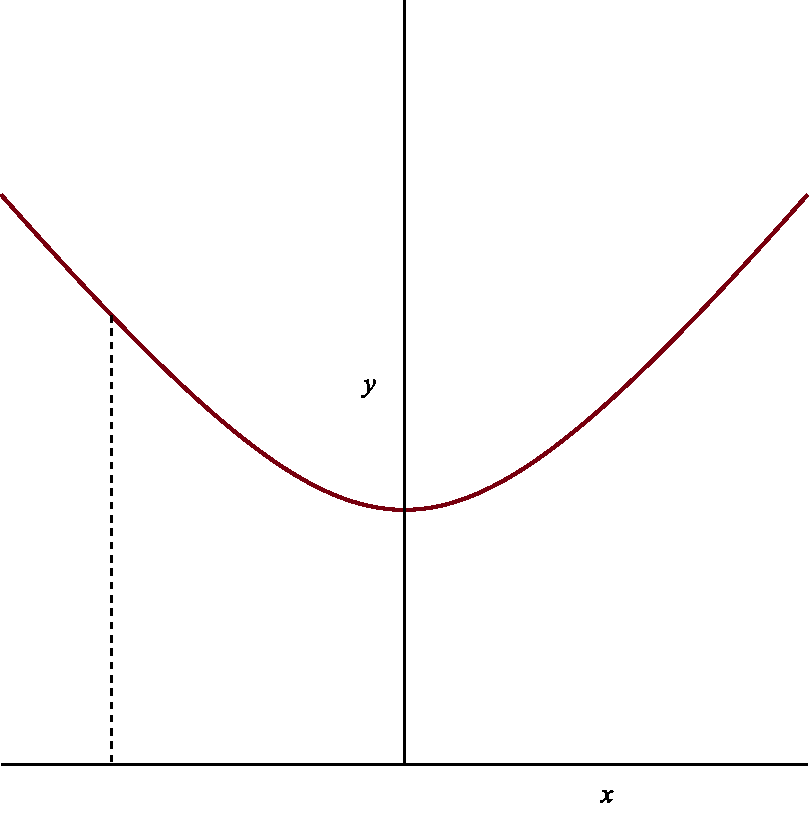
\includegraphics[width=0.6\textwidth]{hyperbola.pdf}
    %\captionsetup{labelformat=empty}
    \caption{$y=\sqrt{1+x^2}$}
  \end{figure}

  \begin{figure}[H]
    \centering
    \def\svgwidth{0.7\columnwidth}
    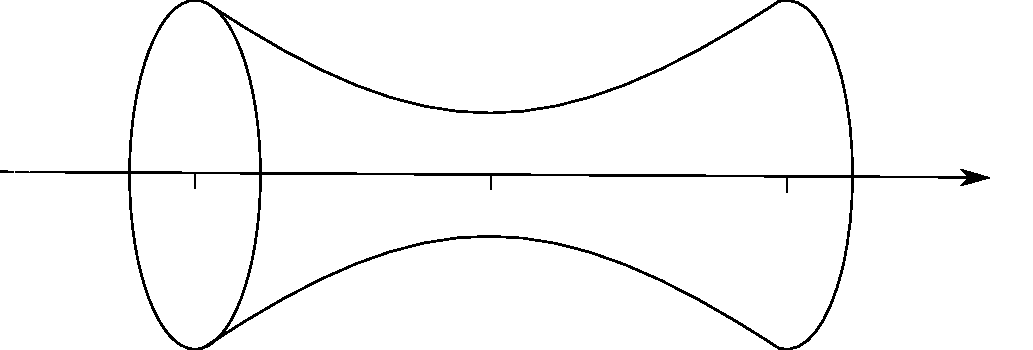
\includegraphics[width=0.6\textwidth]{hyperboloidrev.pdf}
    %\captionsetup{labelformat=empty}
    \caption{Hyperboloid of revolution}
  \end{figure}


As
\[
\dfrac{d y}{d x}=2x\dfrac12(1+x^2)^{-\frac12}=\dfrac x{\sqrt{1+x^2}}
\]
the surface area is
\begin{eqnarray*}
A(-a,a)
&=&2\pi \int_{-a}^a y\sqrt{1+\left(\dfrac{d y}{d x}\right)^2}\ dx\\
&=&2\pi \int_{-a}^a \sqrt{1+x^2}\sqrt{1+\dfrac {x^2}{1+x^2}}\ dx\\
&=&2\pi \int_{-a}^a \sqrt{1+x^2+x^2}\ dx\\
&=&2\pi \int_{-a}^a \sqrt{1+2x^2}\ dx.
\end{eqnarray*}
Hence, the substitution $u=\sqrt2 x$ yields $du=\sqrt 2 dx$ and so
\begin{eqnarray*}
A(-a,a)
&=&2\pi \int_{-\sqrt2 a}^{\sqrt2 a} \sqrt{1+u^2}\ \dfrac{du}{\sqrt2}\\
&=&\sqrt2\pi \cdot\dfrac12\left[u\sqrt{1+u^2}+\arcsinh(u)\right]_{-\sqrt2 a}^{\sqrt2 a}\\
&=&\sqrt2\pi \left[\sqrt2 a\sqrt{1+2a^2}+\arcsinh(\sqrt2 a)\right].
\end{eqnarray*}
\end{example}


